\documentclass[12pt,letterpaper,oneside]{article}
% The file intend to keep track of good practices in Latex writing.

%==============================
% DOCUMENT
%==============================

% Fix some error reporting
\vfuzz2pt % Don't report over-full v-boxes if over-edge is small
\hfuzz2pt % Don't report over-full h-boxes if over-edge is small

% All the same, there are commands, classes and packages which are outdated and superseded. 
% nag provides routines to warn the user about the use of those.
\usepackage[l2tabu,orthodox]{nag}

%==============================
% BIBLIOGRAPHY
%==============================

% \addbibresource{references.bib} % in your preamble
% \citet{key}, \citep{key} % in the document
% \printbibliography % to generate the reference section
\usepackage[
backend=bibtex8, 
style=ieee, 
sorting=none, 
natbib=true, 
doi=false, 
isbn=false, 
url=false, 
eprint=false, 
maxcitenames=1, 
mincitenames=1
]{biblatex}

%==============================
% TEXT
%==============================

% \autoref{key} % instead of Figure~\ref{key}, Table~\ref{key}, Equation~\ref{key}, or Section~\ref{key}
\usepackage[pdftex,colorlinks]{hyperref}
% fix names for autoref
\def\sectionautorefname{Section}
\def\subsectionautorefname{Section}
\def\subsubsectionautorefname{Section}
\newcommand*{\Appendixautorefname}{Appendix}

% \acrodef{ICP}{Iterative Closest Point} % in the preamble
% \ac{ICP} % in the document
\usepackage[printonlyused]{acronym}

% International unit system 
% e.g., \SI{1000}{\m\squared}, \num{20000}
\usepackage{siunitx}
\sisetup{group-separator = \text{\,}} % small space for thousand separator

% avoid single line on a page or single line under a figure
% no command to use
\usepackage[all]{nowidow}

% Colored text
\usepackage[dvipsnames]{xcolor}

% Fill the template with text
\usepackage{lipsum}

% Better command to make sure that people don't confuse lipsum text with real text
\newcommand{\lightlipsum}[1][0]{\textcolor{gray!50}{\lipsum[#1]}}

%==============================
% FIGURE
%==============================

% Preferred figure format:
% - pdf or eps for graphs and schemas
% - jpg for photo
% Don't use png as each compilation decompress the image, thus making compilation time
% untolerable when there are more than 5 images...

% \includegraphics[width=\textwidth]{filename}
\usepackage[pdftex]{graphicx}

% convert eps to pdf, you need to skip the file extension to work properly
% \includegraphics{filename} % instead of \includegraphics{filename.eps}
\usepackage{epstopdf}

% for Inkscape figures, import tex files in other folder and keep paths coherent
% e.g., \import{images}{timeline.pdf_tex}
\usepackage{import}

% include path for logos
\graphicspath{{./figures/}}

%==============================
% TABLE
%==============================

% Cleaner spacing for tables
% \toprule, \midrule, \bottomrule % instead of \hline
\usepackage{booktabs}

% Tables that can fit page length
% e.g.,three columns with the second one being twice as large as the others
% \begin{tabu}{X X[2] X}
\usepackage{tabu}

%==============================
% MATH
%==============================

% Better symboles
\usepackage{amssymb,amsfonts,amsmath,amscd}

% \bm % in equations for proper bold font
\usepackage{bm} 

% Some handy commands
\newcommand{\norm}[1]{\left\Vert#1\right\Vert}
\newcommand{\abs}[1]{\left\vert#1\right\vert}
\newcommand{\set}[1]{\left\{#1\right\}}
\newcommand{\Real}{\mathbb R}
\newcommand{\bbm}{\begin{bmatrix}}
\newcommand{\ebm}{\end{bmatrix}}




% ---------------------------------------------------------------
% Load style
%----------------------------------------
% Page style

% Set the page size
\addtolength{\hoffset}{-0.75in} \addtolength{\voffset}{-0.75in}
\setlength{\textwidth}{7in} \setlength{\textheight}{8.25in}
\setlength{\headheight}{0.6in}
\setlength{\headsep}{0.2in}

\setlength{\footskip}{40pt}
\setlength{\fboxsep}{12pt}

% Set the paragraph skip
\setlength{\parskip}{3pt}

% Access to a counter for the number of pages
\usepackage{lastpage}

% To allow text justify on the right
\usepackage{ragged2e}

%----------------------------------------
% Title style

\newcommand{\makeCustomTitle}
{
\begin{center}
\LARGE{\textbf{\reportTitle{}}}
\\
\vspace{5pt}
\normalsize{\reportAuthors{}}
\\
\reportDate{}
\end{center}
\begin{flushright}
\footnotesize{
\begin{tabu}{ccX}
\toprule
\emph{Version} & \emph{Date} & \emph{Comments} \\
\midrule
\reportVersions{} \\
\bottomrule
\end{tabu}
}
\end{flushright}
}

%----------------------------------------
% Section style
\usepackage{sectsty}

% Set the section labeling font
\allsectionsfont{\textsf\bfseries}

%----------------------------------------
% Caption style
\usepackage[font=small, labelfont=bf, skip=5pt]{caption}

%----------------------------------------
% header style
\usepackage{fancyhdr}



% Define the title page style
\fancypagestyle{titlePage}{%
\fancyhf{}%

\fancyhead[L]{
\includegraphics[height=0.45in]{UL_N}}
\fancyhead[C]{\raisebox{0.2in}{\textsc{Technical Report}}}
\fancyhead[R]{
\includegraphics[height=0.45in]{norlab_logo_acronym_dark}}
\fancyfoot[C]{\thepage/\pageref*{LastPage}}

\renewcommand{\headrulewidth}{0.1pt}
\renewcommand{\footrulewidth}{0.2pt}
}

% Define the page style for the other pages
\fancypagestyle{plain}{%
\fancyhf{}
\fancyhead[L]{\reportTitle{}}
\fancyfoot[C]{\thepage/\pageref*{LastPage}}
\renewcommand{\headrulewidth}{0.1pt}
\renewcommand{\footrulewidth}{0.1pt}
}

% Set the page style for all the document except the first page
\pagestyle{plain}

%----------------------------------------
% footnote style
\usepackage{fnpos}
% Fix the footnotes location
\makeFNbottom \makeFNbelow

% ---------------------------------------------------------------
% Author

\author{\reportAuthors{} \\
       Laval University\\
       1065, av. de la Médecine \\
       Quebec, Qc \\
       Canada G1V 0A6 \\
}

% ---------------------------------------------------------------
% PDF setup
\hypersetup{
    pdftitle={\reportTitle},
    pdfauthor={\@author},
    pdfkeywords={research, project, robotics, norlab, Northern Robotics Lab, Master's},
    pdfsubject={},
    pdfstartview={},
    urlcolor=cyan,
    linkcolor=red,
}
% ---------------------------------------------------------------


% Add your other packages here
% make sure to check prembule.tex first!
\usepackage{wrapfig}
\usepackage{biblatex}


%================================================================
\bibliography{bibliography}
\begin{document}
\thispagestyle{empty}	% Pour éviter d'avoir un en-tête et un pied de page sur la page couverture

\includegraphics[width=5cm]{../figures/logoUlaval.jpg}	% Pour inclure le logo (on précise la largeur de l'image)
\hspace{4.5cm}

\includegraphics[width=7cm]{../figures/norlab_logo_acronym_dark.png}
\vspace{1cm}	% Espacement vertical

\begin{center}	% On centre le texte
{\huge \textbf{\ Marmotte \\ HD2 Robot platform \\ Technical Document}}\\ % \huge fait que le texte est gros, \bf fait que le texte est gras
\large
\vspace{1cm}
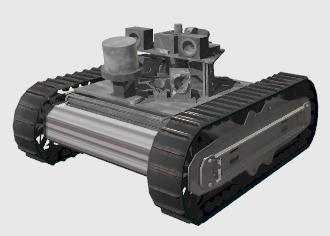
\includegraphics[width=5cm]{../figures/marmotteCAD1.png}
\vspace{1cm}

Presented to NORLab for SubT \\ DARPA competition


\vspace{4cm}
by \\ 
Nicolas Antonucci \\
Electrical engineering intern at Norlab

\vfill	% On va jusqu'au bas de la page avant de mettre le texte ci-dessous

%\today
\text{Summer 2021 project}

\pagebreak
\end{center}
%\makeCustomTitle
\thispagestyle{titlePage}

% ---------------------------------------------------------------
\begin{abstract}
Technical document showing the low level electronics as well as the ROS packages used to control the robot with a controller. Design techniques are shown to help reduce electrical noise as much as possible as well as information on some of the electrical connections. Schematics of the PCB designs are provided as well. This document will continue to evolve over the course of summer 2021. I thank you in advance for taking the time to read this document. I will be happy to answer any questions as well as take any feedback on the layout and execution of this document or make any changes if necessary. I can be reached at nicolas.antonucci.1@ulaval.ca.
\end{abstract}

% ---------------------------------------------------------------

\tableofcontents
\listoffigures

% ---------------------------------------------------------------
\newpage
\section{Robot design}

\subsection{Platform}

\begin{wrapfigure}{l}{0.4\textwidth}
  \begin{center}
    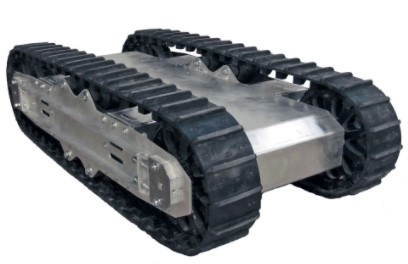
\includegraphics[width=0.38\textwidth]{../figures/platform.jpg}
  \end{center}
  \caption{Platform}
\end{wrapfigure}

This is the HD2 Treaded Tank Robot Platform from superdroidrobots.com \cite{superdroidrobots}. This particular model was chosen because of its robustness and its ability to easily cross many obstacle. One of the main objectives of this robot is to quickly and effectively provide reconnaissance of an unknown erea. Therefore our objectives for low level electronics and control is to have solid electrical connections that will withstand vibrations, heat and electrical noise as well as robust code that will not lag or glitch.\\

The platform is controled through the Roboclaw 2X30A motor controller from basicmicro, \cite{Roboclaw}, \cite{RoboclawData,RoboclawManual}. The motors used are the IG52-04 24VDC 285 RPM Gear Motors, \cite{EncMotors,RegMotors}, 2 of them with encoders. Encoders are not needed for the other 2 as they are connected in line with the same track.

\subsection{Block diagram}

\begin{figure}[h]
    \centering
    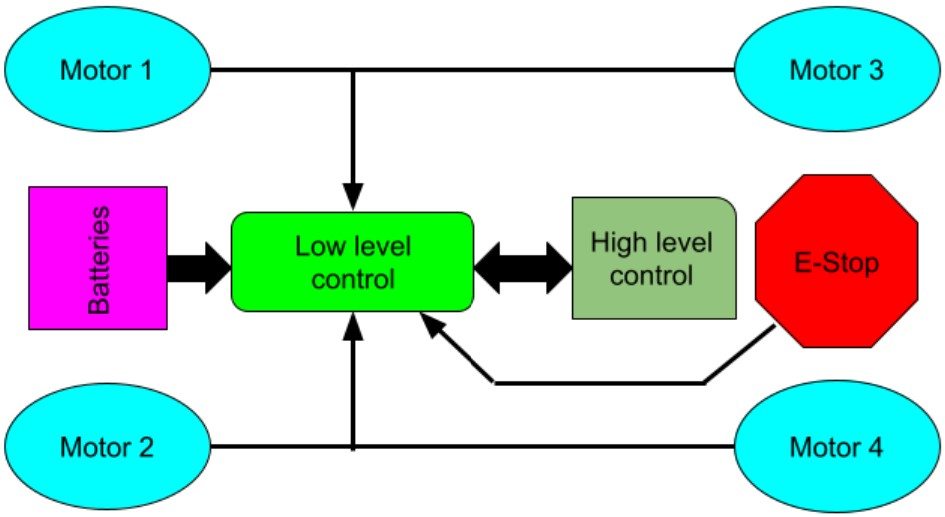
\includegraphics[width=0.8\textwidth]{../figures/blockDiagram.png}
    \caption{Low level block diagram}
    \label{fig:blockl}
\end{figure}

% ---------------------------------------------------------------

\newpage
\section{D.C. Geared motors}

This next table shows the different motor configurations with their respective current draws and we can see our highlighted configuration at the bottom.

\begin{figure}[h]
    \centering
    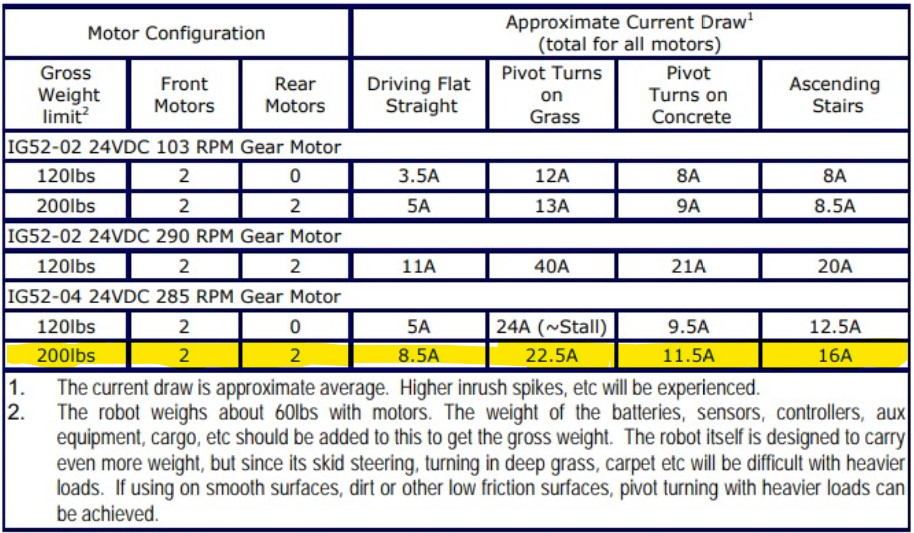
\includegraphics[width=0.7\textwidth]{../figures/motorSpecs.jpg}
    \caption{Motor config}
    \label{fig:motorConfig}
\end{figure}

\begin{wrapfigure}{r}{0.35\textwidth}
  \begin{center}
    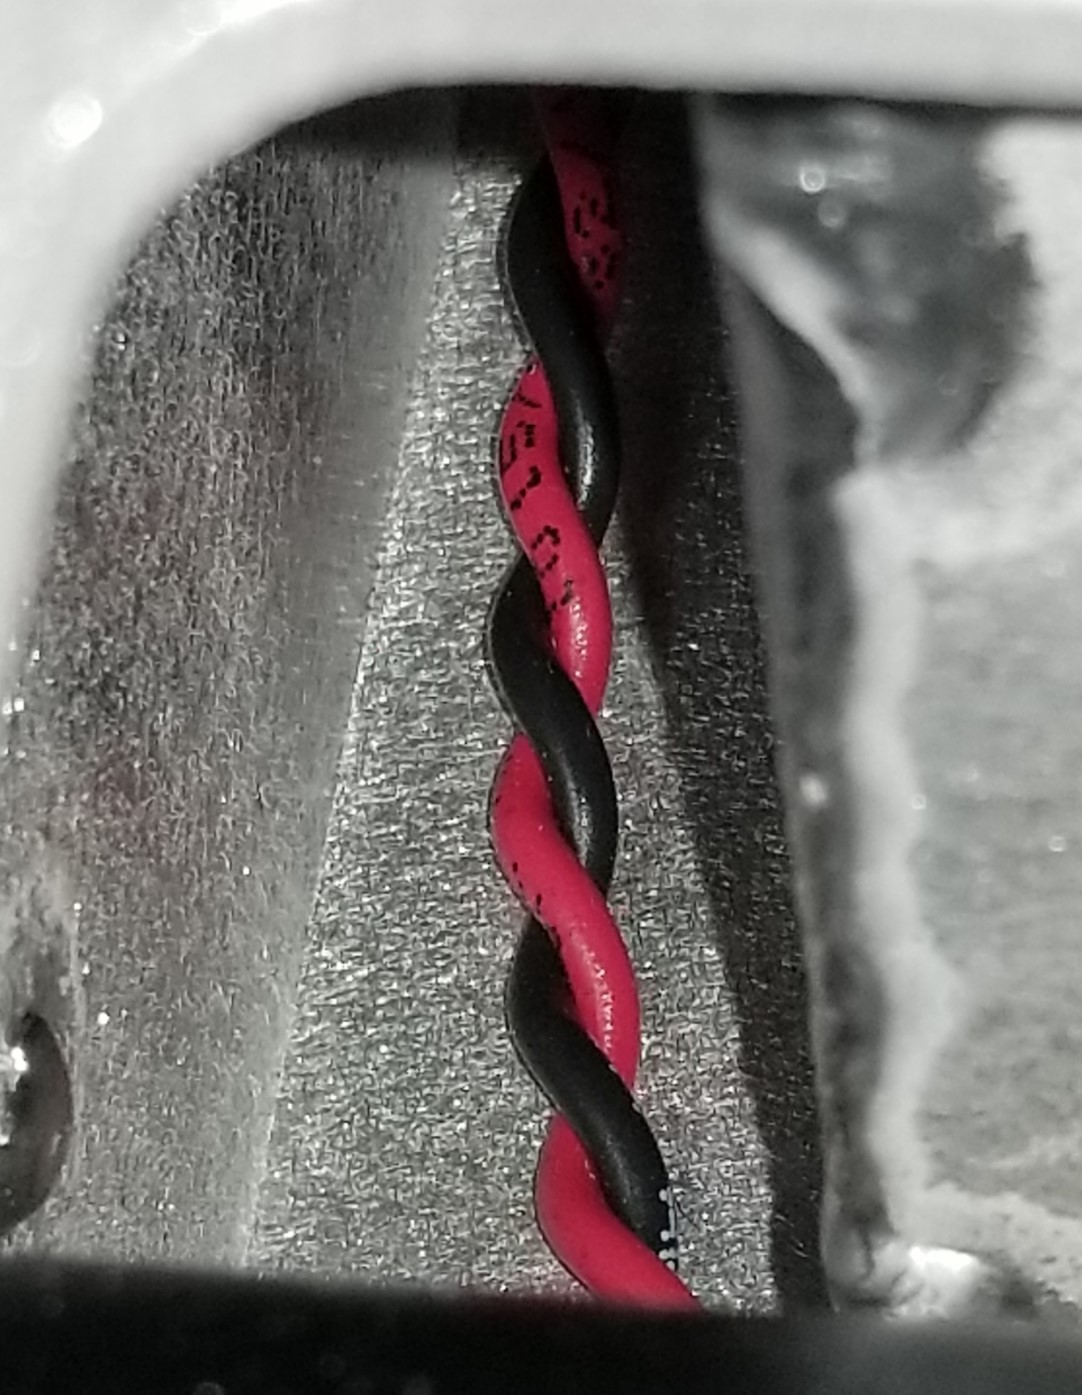
\includegraphics[width=0.34\textwidth]{../figures/twistedMotorWires.jpg}
  \end{center}
  \caption{Motor wires}
\end{wrapfigure}

During the wiring of the motors we were careful to install ferrite beads as close as possible to each motor. We also twisted the positive and negative wire together. These actions help us reduce electrical noise from the motors. The encoders require a $1K\Omega$ pull up resistor to VCC as you can see in the following pictures. We made sure to shrink wrap these connections to ensure a reliable connection. In the following pictures we can also see electrical caracteristics

\begin{tabular}{ c c }
    Motor & Pull up resistor attached \\
    %\hline
     \raisebox{-\totalheight}{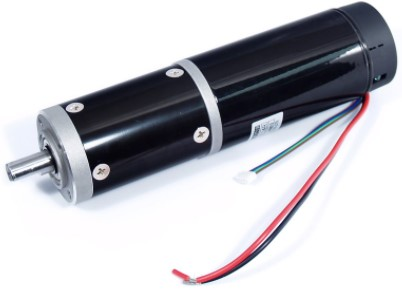
\includegraphics[width=0.45\textwidth]{../figures/motor.jpg}} & \raisebox{-\totalheight}{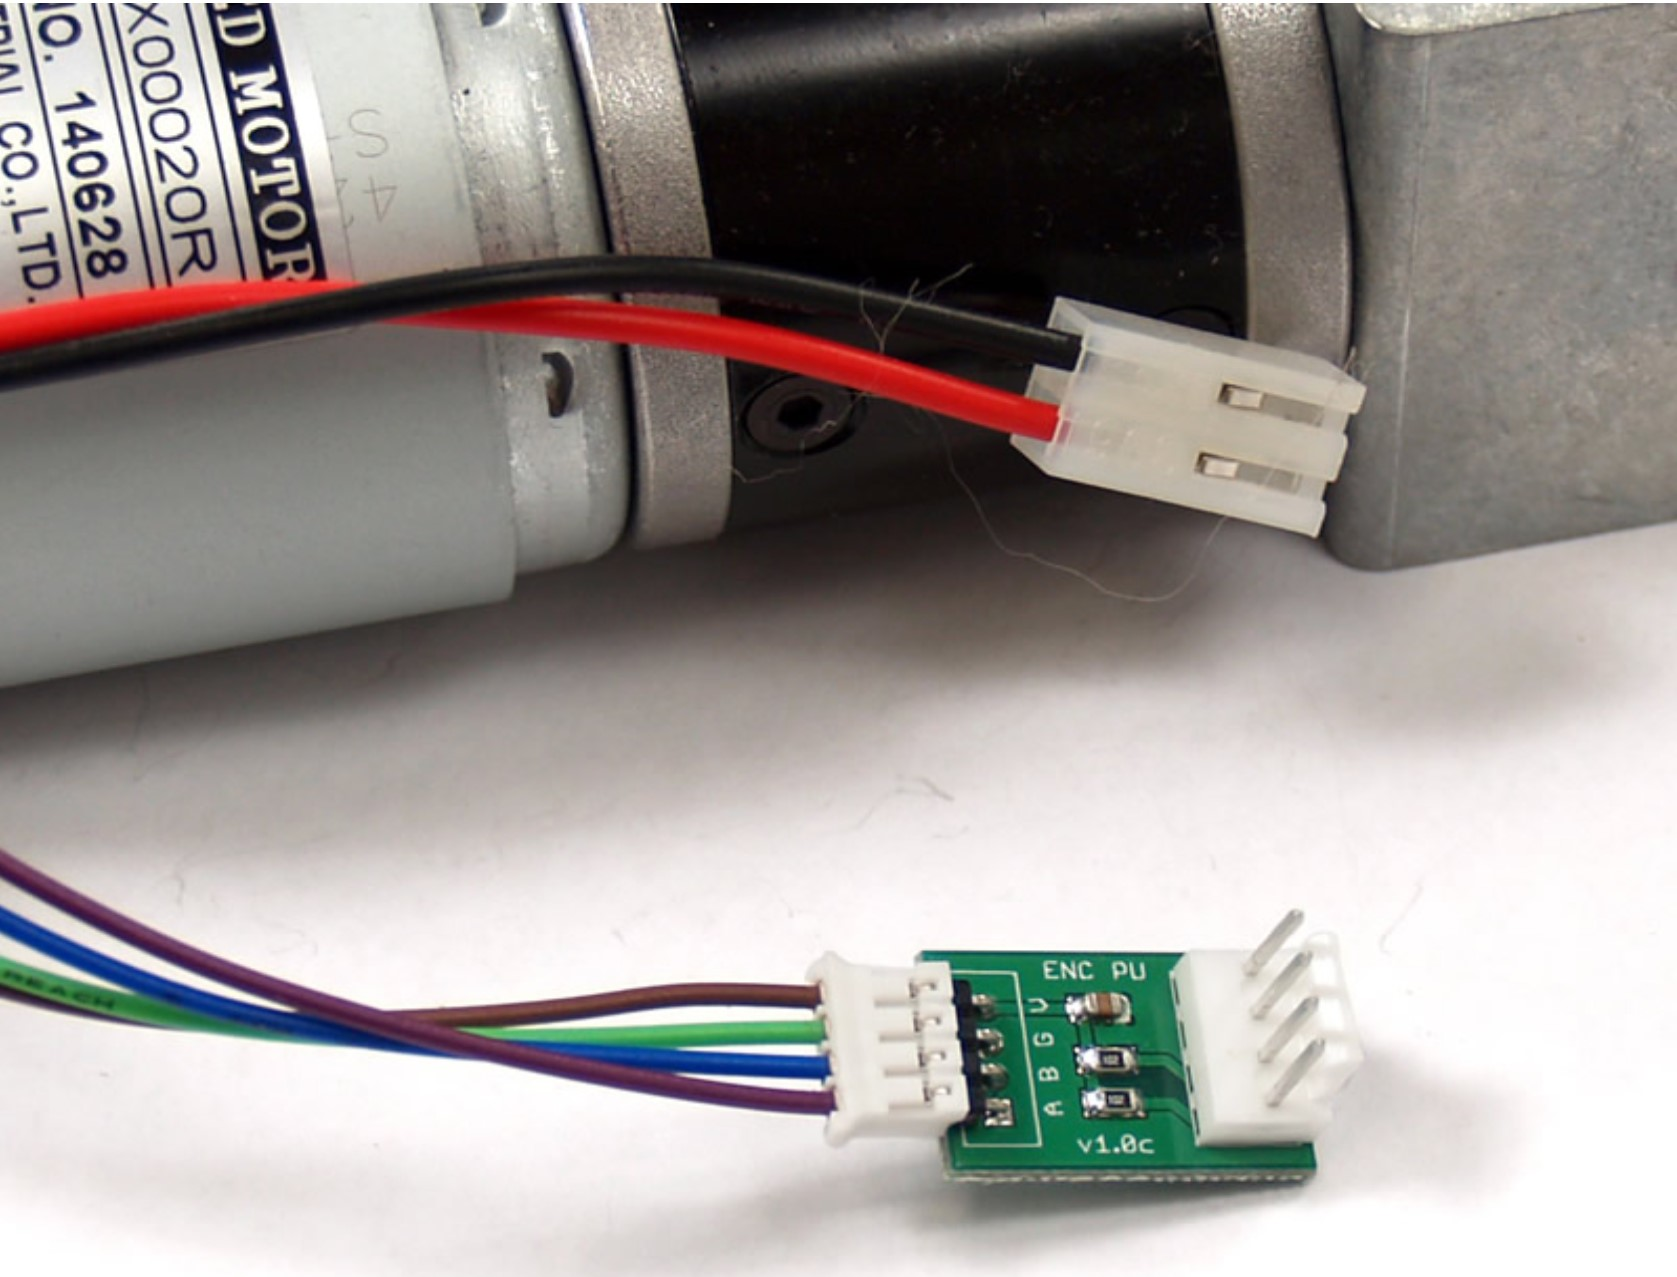
\includegraphics[width=0.45\textwidth]{../figures/gearMotorPullUpBoard.jpg}} \\
\end{tabular}

\begin{tabular}{ c c }
    Cable layout & Schematic \\
    %\hline
     \raisebox{-\totalheight}{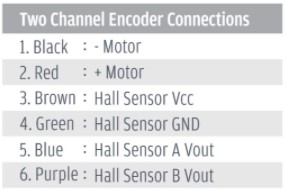
\includegraphics[width=0.45\textwidth]{../figures/encoderPins.jpg}} & \raisebox{-\totalheight}{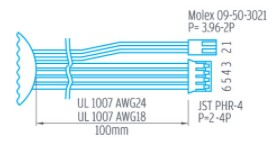
\includegraphics[width=0.45\textwidth]{../figures/encoderPins2.jpg}} \\
\end{tabular}

\begin{tabular}{ c }
    Electrical caracteristics \\
    %\hline
     \raisebox{-\totalheight}{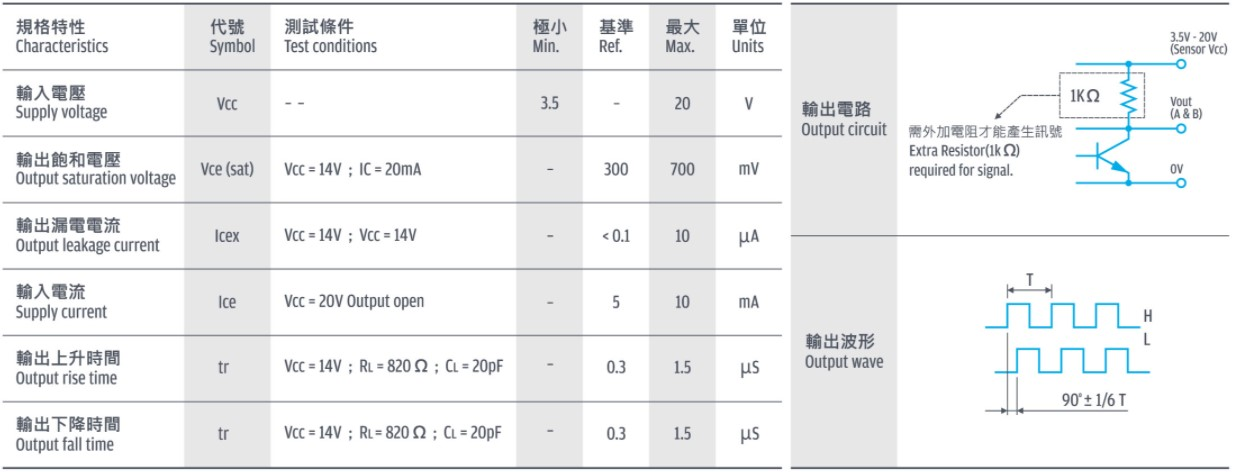
\includegraphics[width=0.9\textwidth]{../figures/electricalCaracteristics.jpg}} \\
\end{tabular}

\begin{itemize}
    \item To reduce noise as much as possible in the system, twist positive and negative wires together and use ferrite beads at each motor connection.
    \item Bigger ferrite first over both wires and one smaller ferrite bead over each wire. (Don't forget the heatshrink)
\end{itemize}


%Here some examples of references \cite{Pomerleau2013,Pomerleau2014}.

% ---------------------------------------------------------------
\newpage
\section{Roboclaw 2x30A Motor Controller}%

\begin{figure}[h]
    \centering
    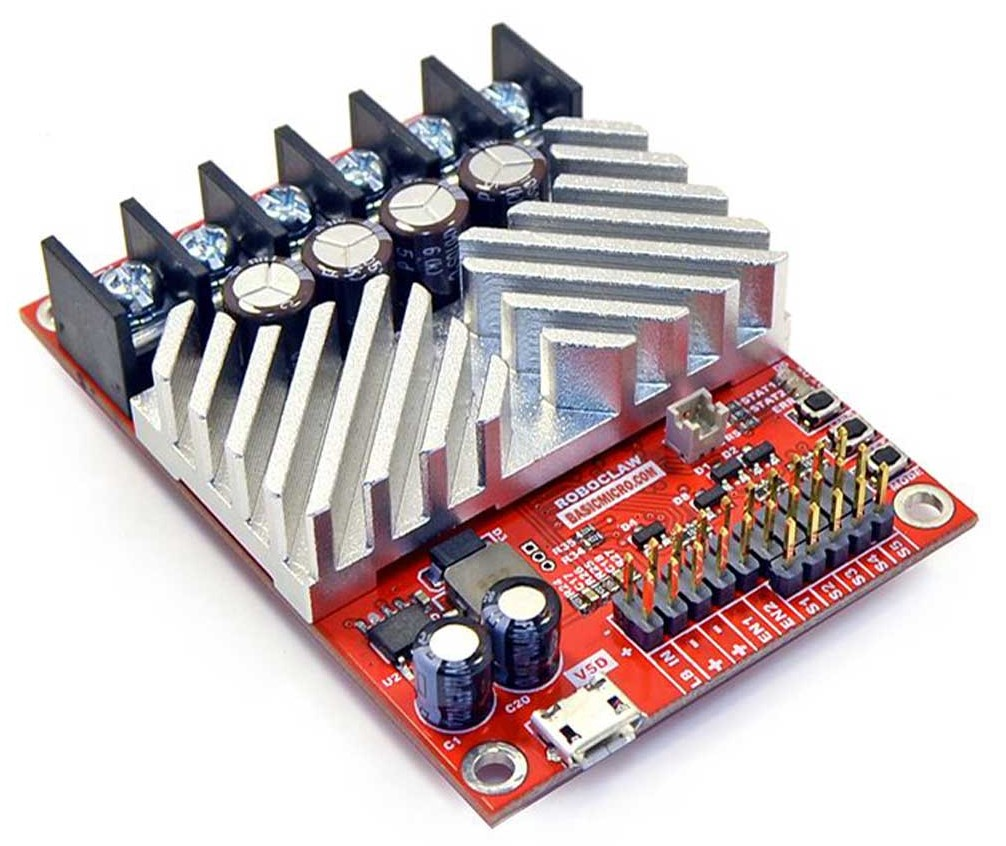
\includegraphics[width=0.3\textwidth]{figures/roboclaw.jpg}
    \caption{Motor Controller}
    \label{fig:my_label}
\end{figure}

\begin{tabular}{ c c }
    Hardware overview & Control interface \\
    %\hline
     \raisebox{-\totalheight}{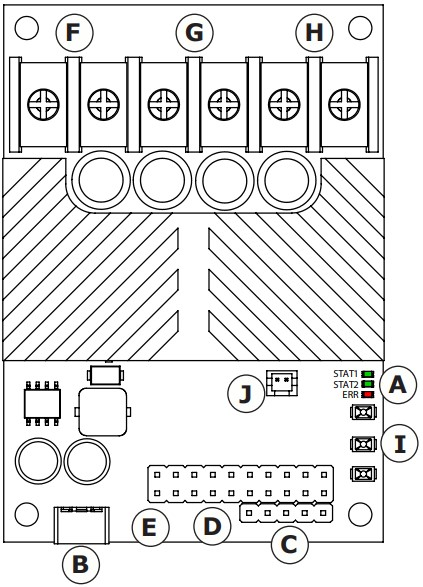
\includegraphics[width=0.30\textwidth]{../figures/roboclawHardwareOverview.jpg}} & \raisebox{-\totalheight}{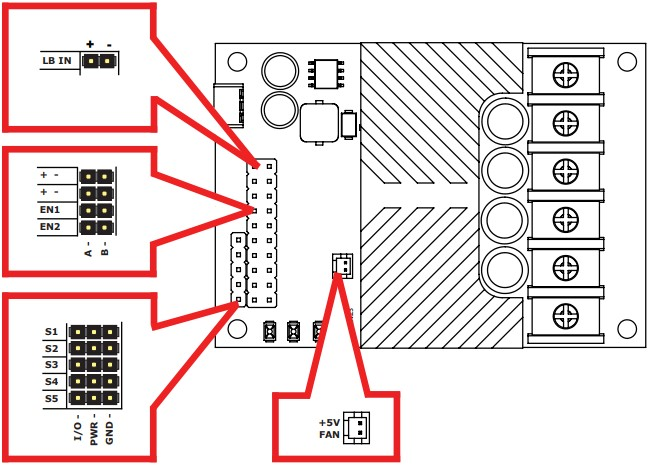
\includegraphics[width=0.55\textwidth]{../figures/roboclawPinLayout.jpg}} \\
\end{tabular}

\begin{itemize}
    \item Connect batteries to the main terminal (G).
    \item Connect encoder through pull up resistor chip to pins in section D.
    \item See schematic below for details.
    \item For initial tests connect roboclaw through usb to computer (batteries have to be connected to roboclaw to function). Use motion studio to check if motors and sensors work.
\end{itemize}

\newpage
\begin{figure}[h]
    \centering
    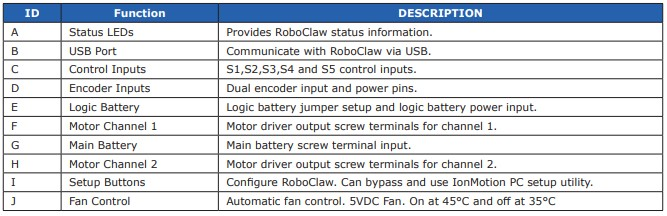
\includegraphics[width=0.9\textwidth]{../figures/roboclawHardwareTable.jpg}
    \caption{Hardware overview reference table}
    \label{fig:my_label}
\end{figure}

\begin{figure}[h]
    \centering
    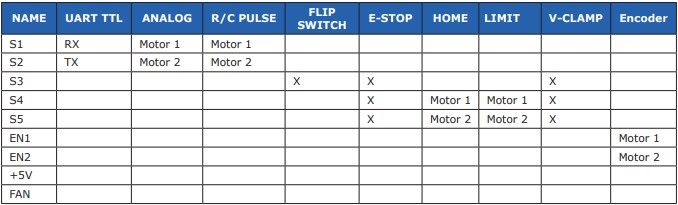
\includegraphics[width=0.9\textwidth]{../figures/roboclawPinTable.jpg}
    \caption{Control interface reference table}
    \label{fig:my_label}
\end{figure}

\newpage
\begin{figure}[h]
    \centering
    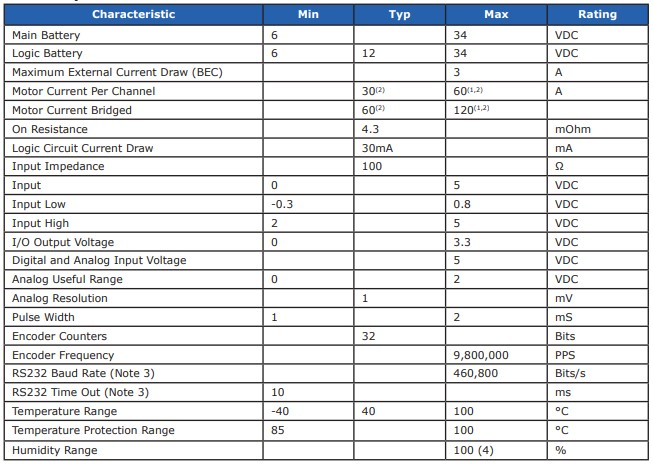
\includegraphics[width=0.9\textwidth]{../figures/electricalSpecsTable.jpg}
    \caption{Electrical specifications}
    \label{fig:my_label}
\end{figure}

\newpage
\begin{figure}[h]
    \centering
    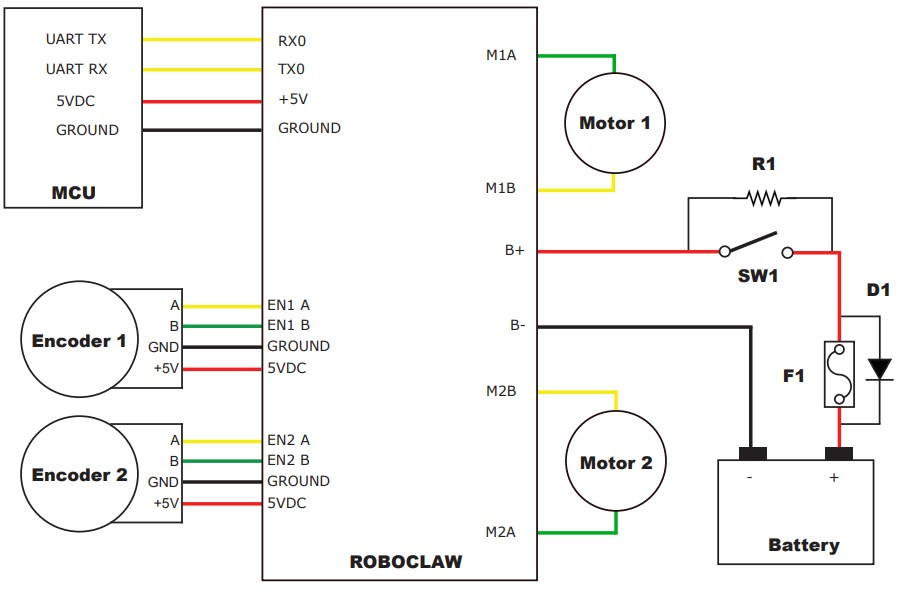
\includegraphics[width=0.9\textwidth]{../figures/wiring.jpg}
    \caption{Safety wiring}
    \label{fig:my_label}
\end{figure}

\section{Motion studio}

\section{ROS Driver}

\section{Remote Control}

% ---------------------------------------------------------------
\newpage
\printbibliography


\end{document}